\section{Introduction}
Cardiomyopathies and arrhythmia are conditions with high morbidity and limited therapies. Although a vast number of genes have been discovered to contribute to the etiology of these diseases, translational research, the practical application of genetic knowledge to improve screening, diagnosis, and treatment for affected individuals and their families has been limited. One major obstacle is the lack of understanding of the relationship between genotype and emergent phenotype, the mechanisms by which pathologies occur, and the identification of factors that cause clinical variability between and within families. Our collaborators in the Grosberg and Zargoza labs are currently studying three affected families each with different mutation in the Lamin A/C (LMNA) gene.  LMNA, together with LMNB1 and LMNB2, encode the main proteins of the nuclear lamina, the structural matrix of the nuclear envelope that interacts with both chromatin in the cell nucleus and the cytoskeleton ~\cite{Capell2006}. In their experiments, it has been obserbed that the nuclei often have a wide variety of geometrical defects, including rounded protrusions which we will refer to as nuclear blebs, as in Fig. ~\ref{fig::blebnuclei}. This is a known property of LMNA mutated cell lines (such as in progeria), however the mechanisms by which such defects forms are unclear. It is known that the LMNA mutation impacts the nuclear lamina, which is present at the inner layer of the nuclear membrane. As a key component of the nuclear lamina, lamin plays an important role in nucleus-cytoplasm interaction and signaling through lamin-binding protein complexes including SUN and KASH that span the nuclear membrane ~\cite{Ho2012}. Cells in this line of experiments come from patients with heart disease (i.e., cardiomyopathy and/or arrhythmias), and they exhibit a mutation in a gene that is known to correlate with nuclear defects. In addition, our collaborators have control cells from people without heart diseases from the same family as the patients' cells.  Nuclei from both patient and control cell lines have been imaged, and  a variety of nuclear shapes in the two types of cells has been found. Nuclear blebbing involves dynamic, complex interactions among many elements: The nuclear lamina, nuclear membrane, membrane-lamin linkers, and chromatin. Preliminary studies have found that both control (fibroblasts of human origin with no mutation) and patient (fibroblasts from patients with the mutation) exhibit some number of defects. We hypothesize a correlation between nuclear shape types and cardiomyopathies and arrhythmias. Therefore we have an ideal system in which to investigate a possible correlation between specific nuclear defects and disease states.

We will use mathematical modelling to test the hypothesis that abnormal nuclear shapes in patients arise due to a mechanical anomaly in the lamin protein due to the mutation in LMNA. this will allow us to differentiate between the type of defects expected under normal biological variability vs. in a pathological situation. 

\begin{figure}[h]
\centering
\captionsetup{width=.9\linewidth}
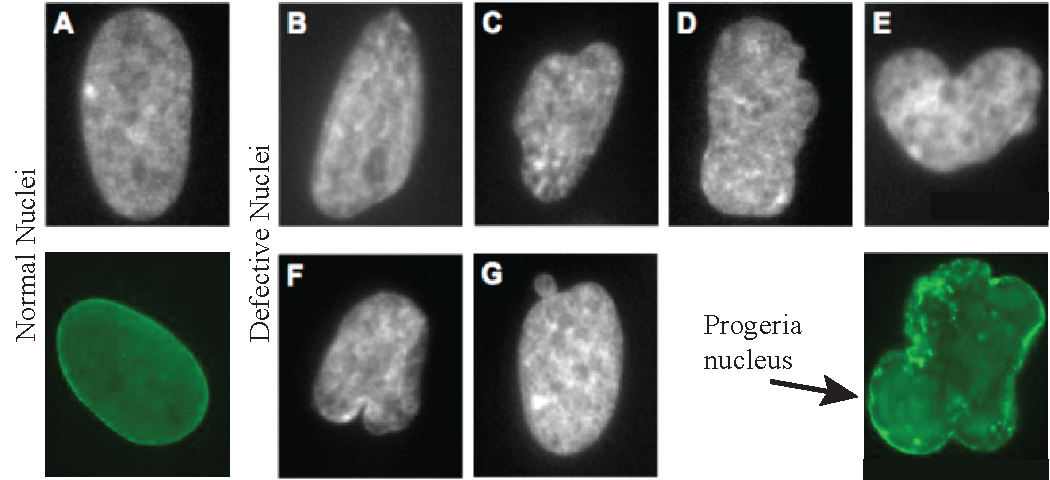
\includegraphics[width=6in]{Project3/figs/blebnuclei}
\caption{Defective nuclei have an irregular shape as compared to normal nuclei. In particular, there may exist one or more protusions at the boundary resulting in a concave nuclei.}
\label{fig::blebnuclei}
\end{figure}
